\startfirstchapter{Results}
\label{chapter:results}

This chapter presents the results of applying the statistical analysis presented in Chapter \ref{chapter:stat} to the MC simulated and observed ATLAS collision events selected for the search\footnote{See Section \ref{sec:evt_selections} for details of the selections applied to define the regions used for the search.}.  


\section{Background-only Fit}

\subsection{Pre- and Post-Fit Yields of MC Simulated Background Events}

\begin{figure}[H]
  \centering
  \begin{subfigure}{0.45\textwidth}
    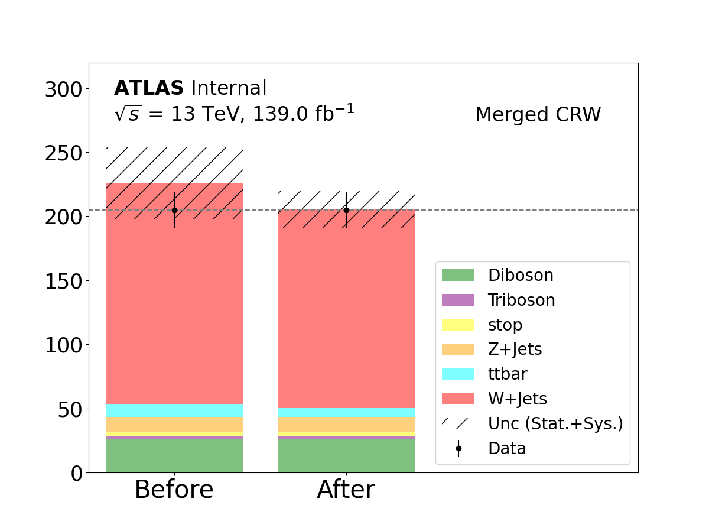
\includegraphics[width=\textwidth]{Figures/8/CRW_Merged_before_after.pdf}
    \caption{Merged CRW}\label{fig:before_after_CRW_merged}
  \end{subfigure} \hspace{1em}
  \begin{subfigure}{0.45\textwidth}
    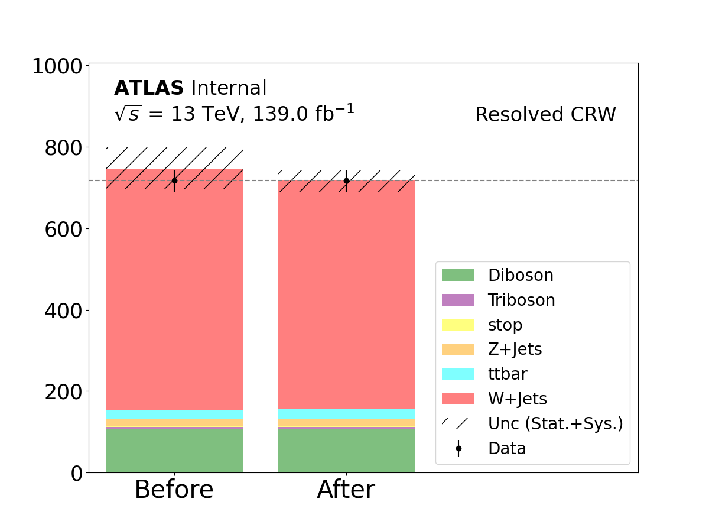
\includegraphics[width=\textwidth]{Figures/8/CRW_Resolved_before_after.pdf}
    \caption{Resolved CRW}\label{fig:before_after_CRW_resolved}
  \end{subfigure} \vspace{1em}
  \begin{subfigure}{0.45\textwidth}
    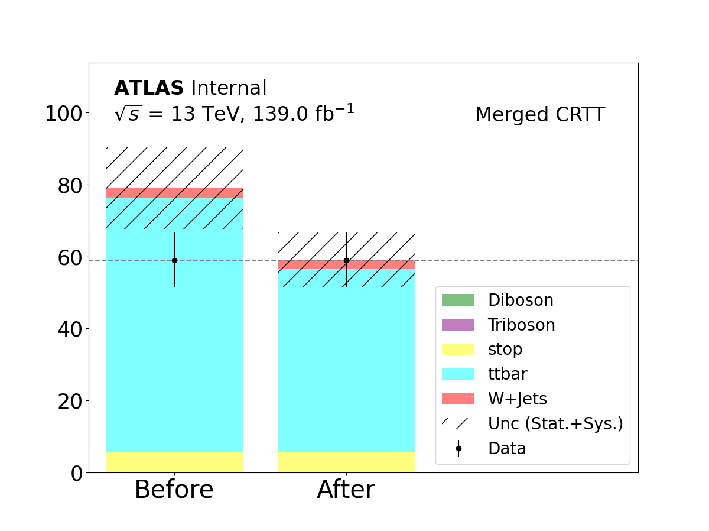
\includegraphics[width=\textwidth]{Figures/8/CRTT_Merged_before_after.pdf}
    \caption{Merged CRTT}\label{fig:before_after_CRTT_merged}
  \end{subfigure} \hspace{1em}
  \begin{subfigure}{0.45\textwidth}
    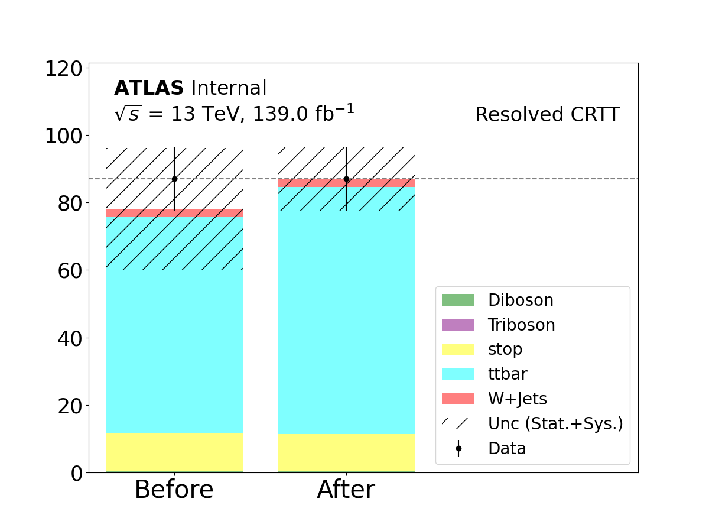
\includegraphics[width=\textwidth]{Figures/8/CRTT_Resolved_before_after.pdf}
    \caption{Resolved CRTT}\label{fig:before_after_CRTT_resolved}
  \end{subfigure} \\ \vspace{1em}
  \caption[]{Comparison between predicted yields of SM background processes and observed yields in the CRs, before and after the background-only fit.}
  \label{fig:before_after_CRs}
\end{figure}

\subsection{Nuisance Parameter Pulls and Correlations}

\begin{figure}[H]
  \centering
  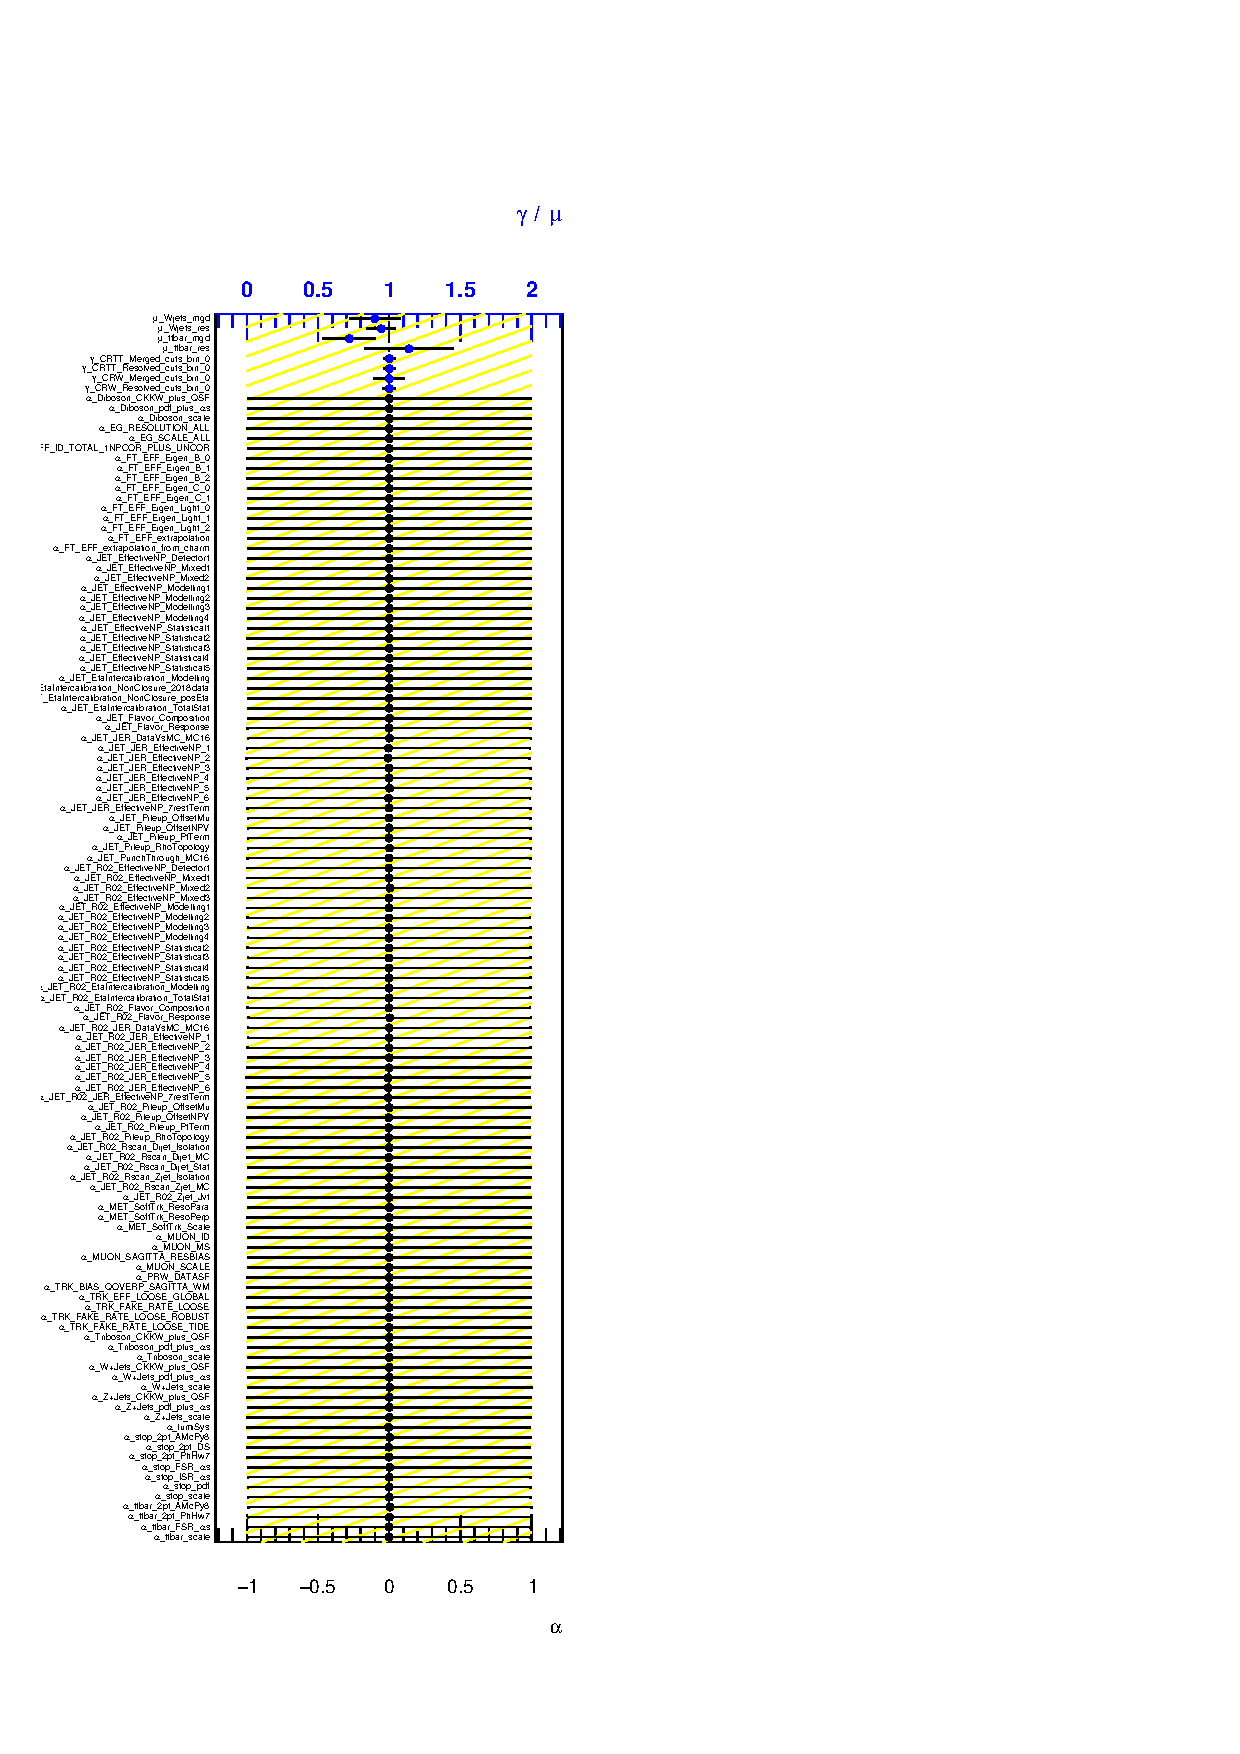
\includegraphics[width=0.55\textwidth]{Figures/8/BkgOnly/fit_parameters.pdf}
  \caption[Pull plots for background-only fit]{\footnotesize{Post-fit values of all NPs in the background-only fit. See Tables \ref{tab:np_naming}, \ref{tab:exp_syst_naming} and \ref{tab:theo_syst_naming} for details of the scheme used to name the NPs. Yellow hatched band shows the pre-fit uncertainty for each NP, and black horizontal error bars show the post-fit uncertainty.}}
  \label{fig:pull_bkgonly}
\end{figure}

\begin{figure}[H]
  \centering
  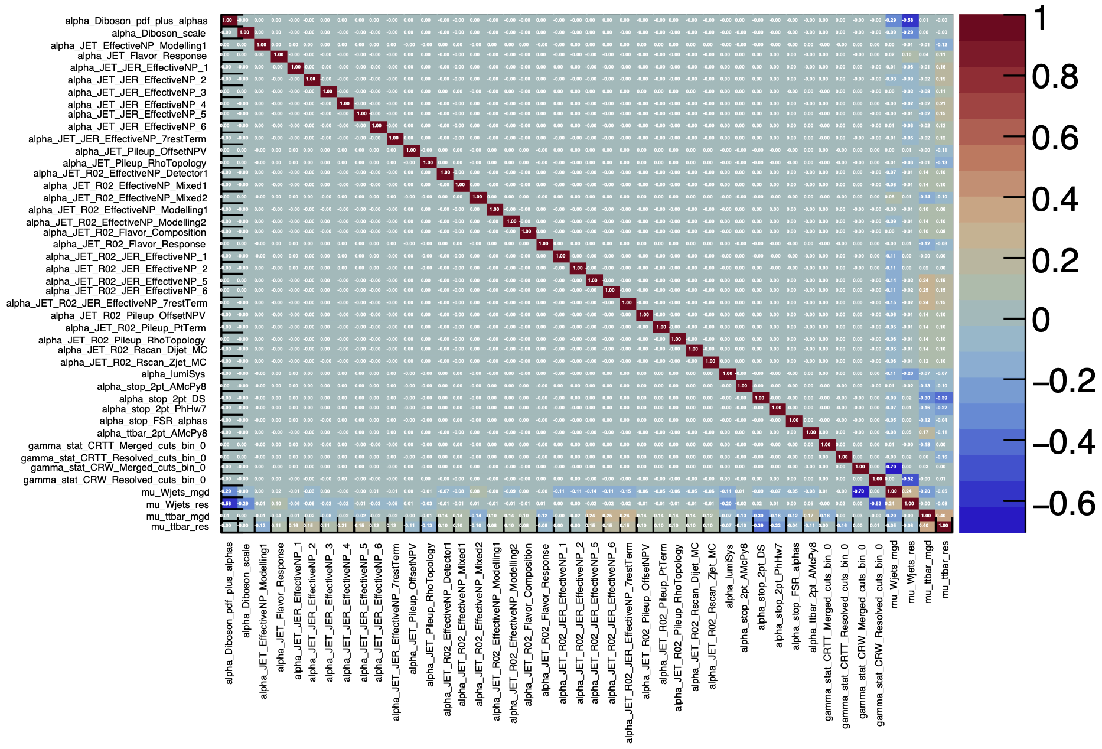
\includegraphics[width=\textwidth]{Figures/8/BkgOnly/c_corrMatrix_RooExpandedFitResult_afterFit_edited.pdf}
  \caption[Pull plots for background-only fit]{\footnotesize{Correlation matrix for all NPs considered in the background-only fit for which at least one correlation coefficient with another NP is larger than 0.1. See Tables \ref{tab:np_naming}, \ref{tab:exp_syst_naming} and \ref{tab:theo_syst_naming} for details of the scheme used to name the NPs.}}
  \label{fig:corrs_bkgonly}
\end{figure}

\section{Comparison of SM Background Expectation and Data in the Signal Region}

\begin{figure}[H]
  \centering
  \begin{subfigure}{0.45\textwidth}
    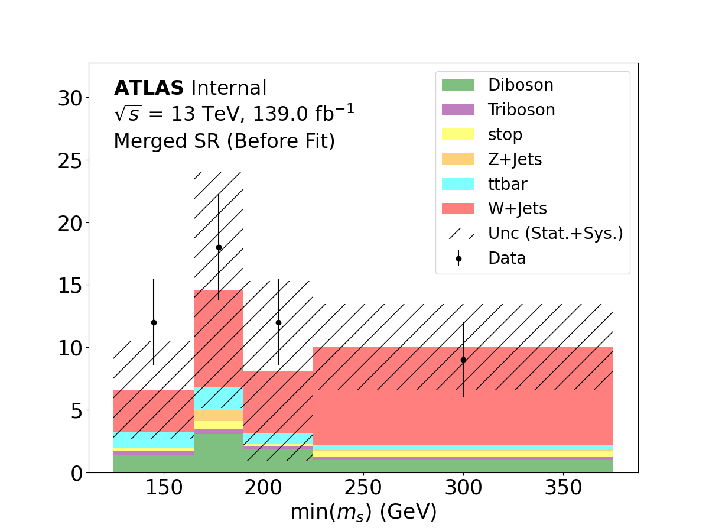
\includegraphics[width=\textwidth]{Figures/8/SR_Merged_before.pdf}
    \caption{Merged SR (Before Fit)}\label{fig:before_SR_merged}
  \end{subfigure} \hspace{1em}
  \begin{subfigure}{0.45\textwidth}
    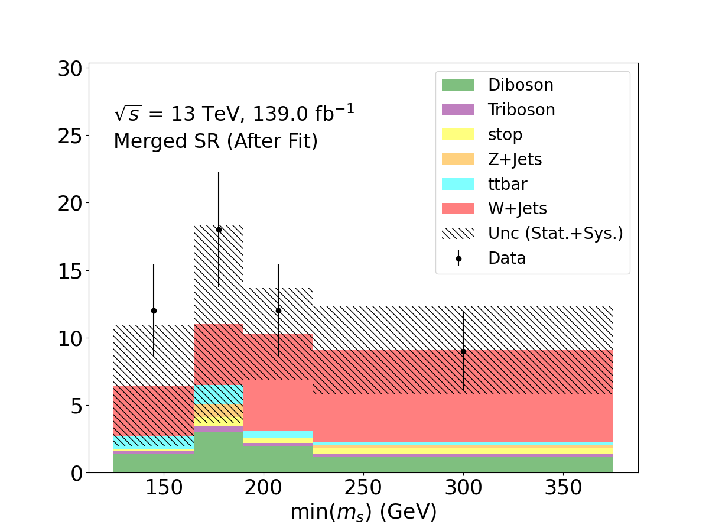
\includegraphics[width=\textwidth]{Figures/8/SR_Merged_after.pdf}
    \caption{Merged SR (After Fit)}\label{fig:after_SR_resolved}
  \end{subfigure} \vspace{1em}
  \begin{subfigure}{0.45\textwidth}
    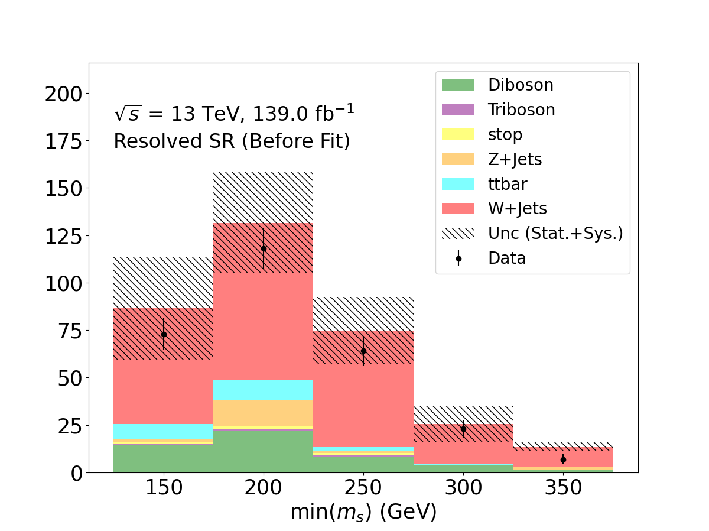
\includegraphics[width=\textwidth]{Figures/8/SR_Resolved_before.pdf}
    \caption{Resolved SR (Before Fit)}\label{fig:before_SR_merged}
  \end{subfigure} \hspace{1em}
  \begin{subfigure}{0.45\textwidth}
    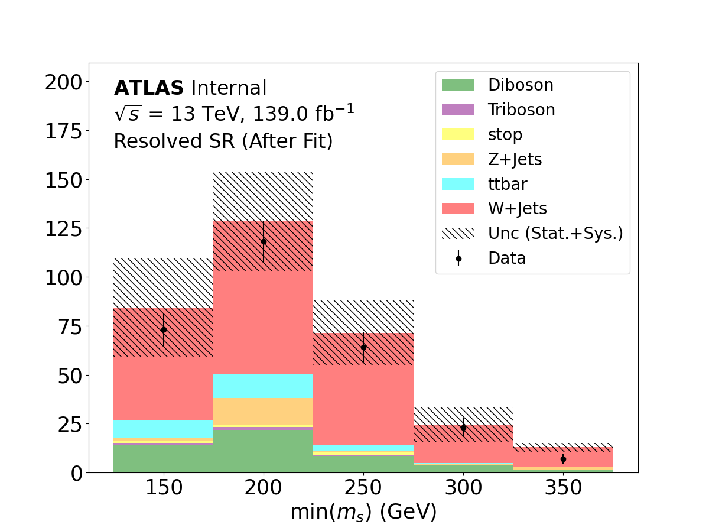
\includegraphics[width=\textwidth]{Figures/8/SR_Resolved_after.pdf}
    \caption{Resolved SR (After Fit)}\label{fig:after_SR_merged}
  \end{subfigure} \\ \vspace{1em}
  \caption[]{Comparison between predicted yields of SM background processes and observed yields in the SRs, before (left) and after (right) the background-only fit and extrapolation to the SR.}
  \label{fig:before_after_SRs}
\end{figure}

\section{Exclusion of the Dark Higgs Signal Model}

\subsection{Signal+Background Fit}

\begin{figure}[H]
  \centering
  \begin{subfigure}{0.45\textwidth}
    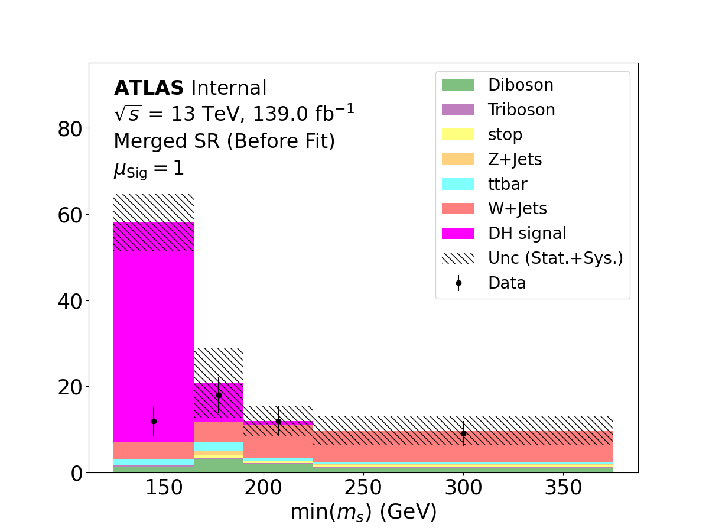
\includegraphics[width=\textwidth]{Figures/8/MonoSlep_monoSWWsemilep_zp1000_dm200_dh160/SR_Merged_before.pdf}
    \caption{Merged SR (Before Fit)}\label{fig:before_SR_merged_MonoSlep_monoSWWsemilep_zp1000_dm200_dh160}
  \end{subfigure} \hspace{1em}
  \begin{subfigure}{0.45\textwidth}
    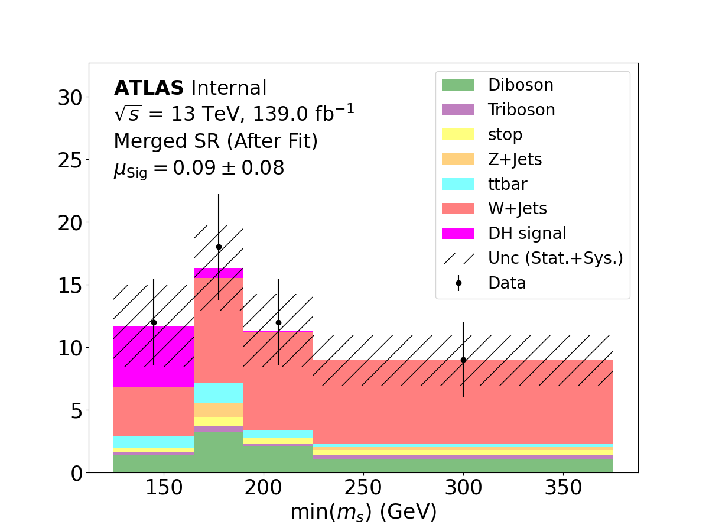
\includegraphics[width=\textwidth]{Figures/8/MonoSlep_monoSWWsemilep_zp1000_dm200_dh160/SR_Merged_after.pdf}
    \caption{Merged SR (After Fit)}\label{fig:after_SR_resolved_MonoSlep_monoSWWsemilep_zp1000_dm200_dh160}
  \end{subfigure} \vspace{1em}
  \begin{subfigure}{0.45\textwidth}
    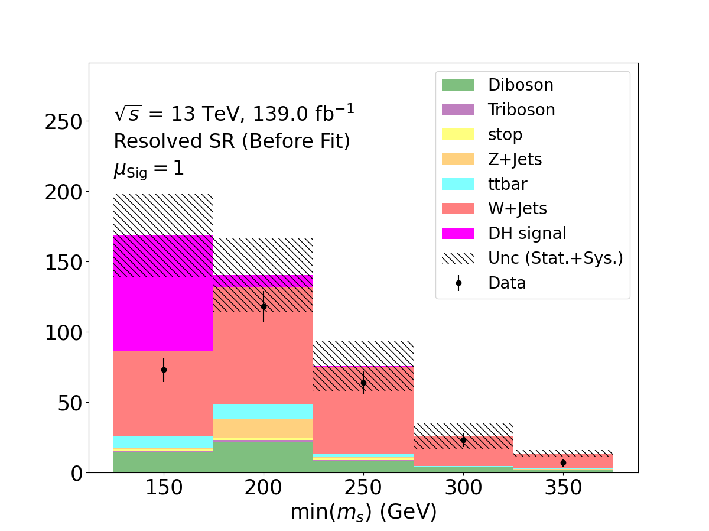
\includegraphics[width=\textwidth]{Figures/8/MonoSlep_monoSWWsemilep_zp1000_dm200_dh160/SR_Resolved_before.pdf}
    \caption{Resolved SR (Before Fit)}\label{fig:before_SR_merged_MonoSlep_monoSWWsemilep_zp1000_dm200_dh160}
  \end{subfigure} \hspace{1em}
  \begin{subfigure}{0.45\textwidth}
    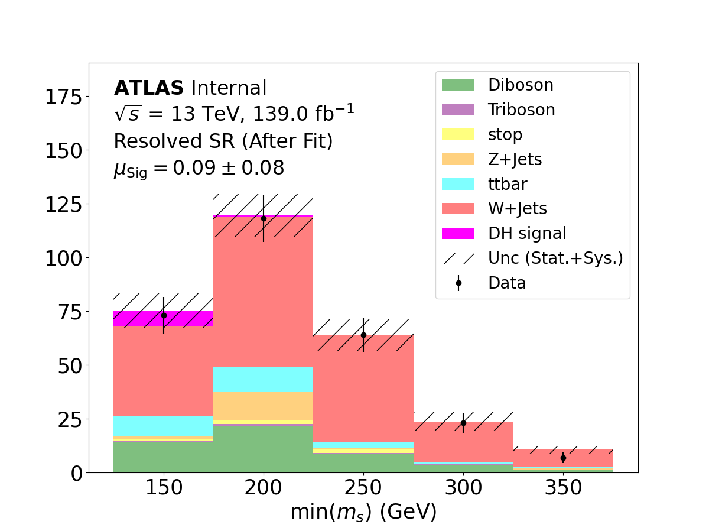
\includegraphics[width=\textwidth]{Figures/8/MonoSlep_monoSWWsemilep_zp1000_dm200_dh160/SR_Resolved_after.pdf}
    \caption{Resolved SR (After Fit)}\label{fig:after_SR_merged_MonoSlep_monoSWWsemilep_zp1000_dm200_dh160}
  \end{subfigure} \\ \vspace{1em}
  \caption[]{Comparison between predicted yields of SM background processes, the DH signal process at \((\ms, \mZp) = (160, 1000)~\GeV\) and observed yields in the SRs. Yields are shown before (left) and after (right) the signal+background fit.}
  \label{fig:before_after_SRs_MonoSlep_monoSWWsemilep_zp1000_dm200_dh160}
\end{figure}

\begin{figure}[H]
  \centering
  \begin{subfigure}{0.45\textwidth}
    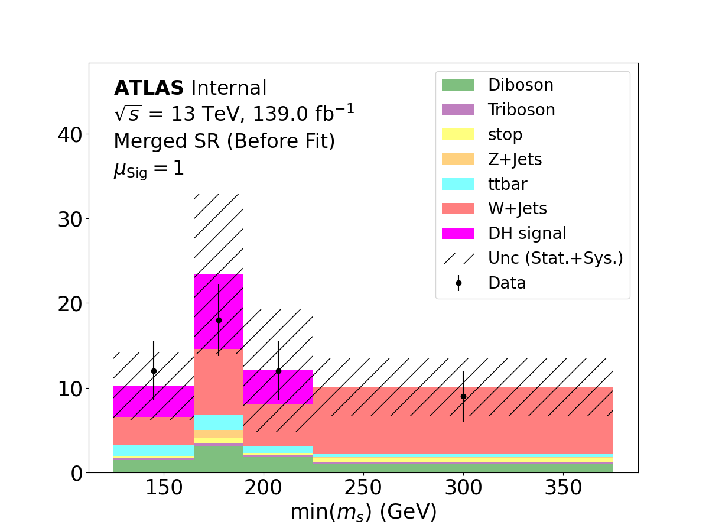
\includegraphics[width=\textwidth]{Figures/8/MonoSlep_monoSWWsemilep_zp2100_dm200_dh210/SR_Merged_before.pdf}
    \caption{Merged SR (Before Fit)}\label{fig:before_SR_merged_MonoSlep_monoSWWsemilep_zp2100_dm200_dh210}
  \end{subfigure} \hspace{1em}
  \begin{subfigure}{0.45\textwidth}
    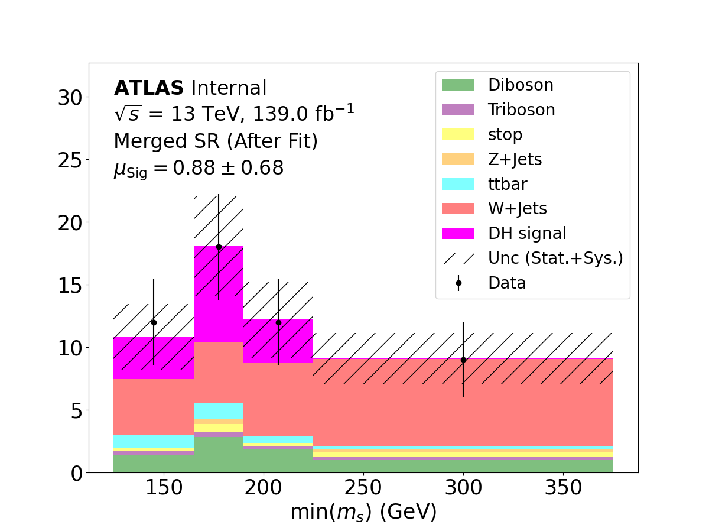
\includegraphics[width=\textwidth]{Figures/8/MonoSlep_monoSWWsemilep_zp2100_dm200_dh210/SR_Merged_after.pdf}
    \caption{Merged SR (After Fit)}\label{fig:after_SR_resolved_MonoSlep_monoSWWsemilep_zp2100_dm200_dh210}
  \end{subfigure} \vspace{1em}
  \begin{subfigure}{0.45\textwidth}
    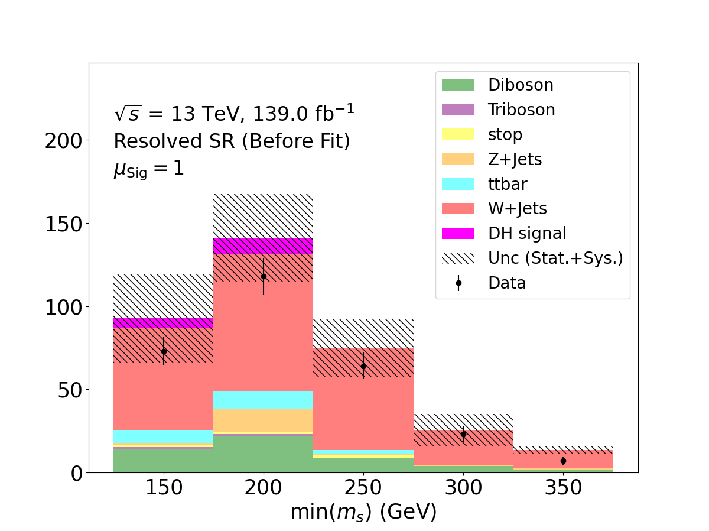
\includegraphics[width=\textwidth]{Figures/8/MonoSlep_monoSWWsemilep_zp2100_dm200_dh210/SR_Resolved_before.pdf}
    \caption{Resolved SR (Before Fit)}\label{fig:before_SR_merged_MonoSlep_monoSWWsemilep_zp2100_dm200_dh210}
  \end{subfigure} \hspace{1em}
  \begin{subfigure}{0.45\textwidth}
    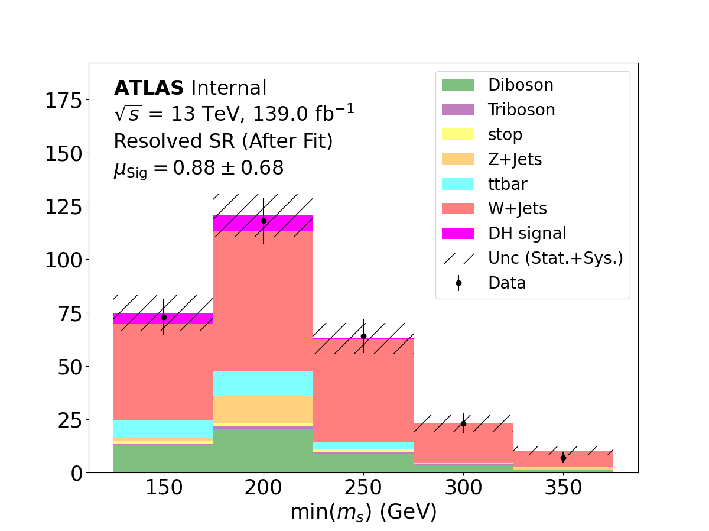
\includegraphics[width=\textwidth]{Figures/8/MonoSlep_monoSWWsemilep_zp2100_dm200_dh210/SR_Resolved_after.pdf}
    \caption{Resolved SR (After Fit)}\label{fig:after_SR_merged_MonoSlep_monoSWWsemilep_zp2100_dm200_dh210}
  \end{subfigure} \\ \vspace{1em}
  \caption[]{Comparison between predicted yields of SM background processes, the DH signal process at \((\ms, \mZp) = (210, 2100)~\GeV\) and observed yields in the SRs. Yields are shown before (left) and after (right) the signal+background fit.}
  \label{fig:before_after_SRs_MonoSlep_monoSWWsemilep_zp2100_dm200_dh210}
\end{figure}

\begin{figure}[H]
  \centering
  \begin{subfigure}{0.45\textwidth}
    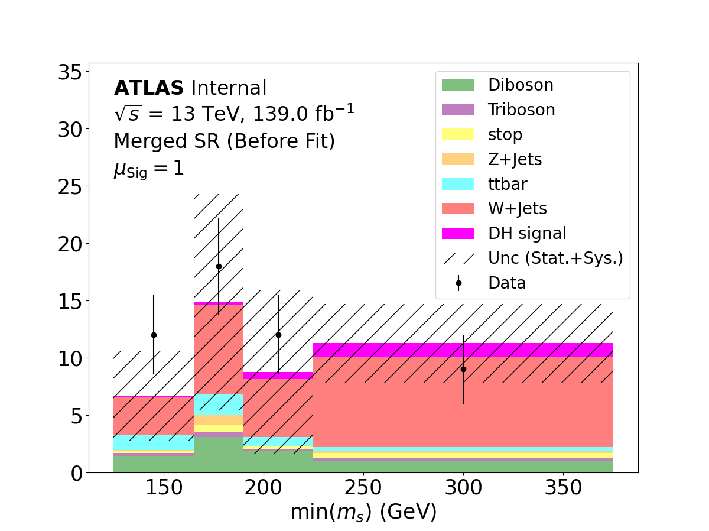
\includegraphics[width=\textwidth]{Figures/8/MonoSlep_monoSWWsemilep_zp2900_dm200_dh310/SR_Merged_before.pdf}
    \caption{Merged SR (Before Fit)}\label{fig:before_SR_merged_MonoSlep_monoSWWsemilep_zp2900_dm200_dh310}
  \end{subfigure} \hspace{1em}
  \begin{subfigure}{0.45\textwidth}
    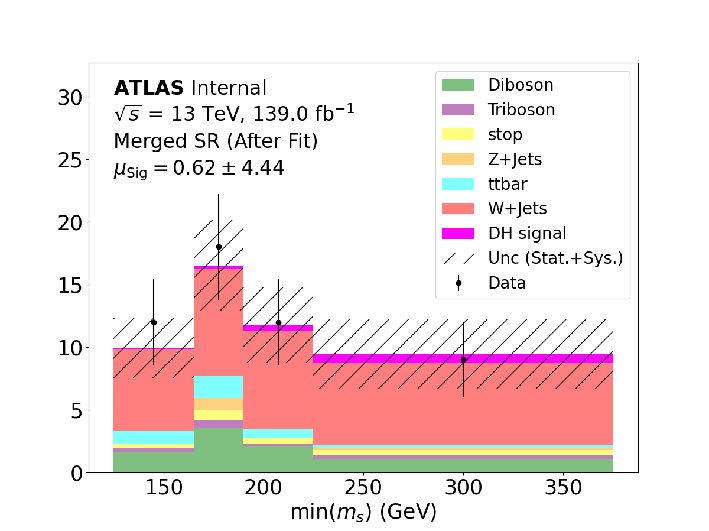
\includegraphics[width=\textwidth]{Figures/8/MonoSlep_monoSWWsemilep_zp2900_dm200_dh310/SR_Merged_after.pdf}
    \caption{Merged SR (After Fit)}\label{fig:after_SR_resolved_MonoSlep_monoSWWsemilep_zp2900_dm200_dh310}
  \end{subfigure} \vspace{1em}
  \begin{subfigure}{0.45\textwidth}
    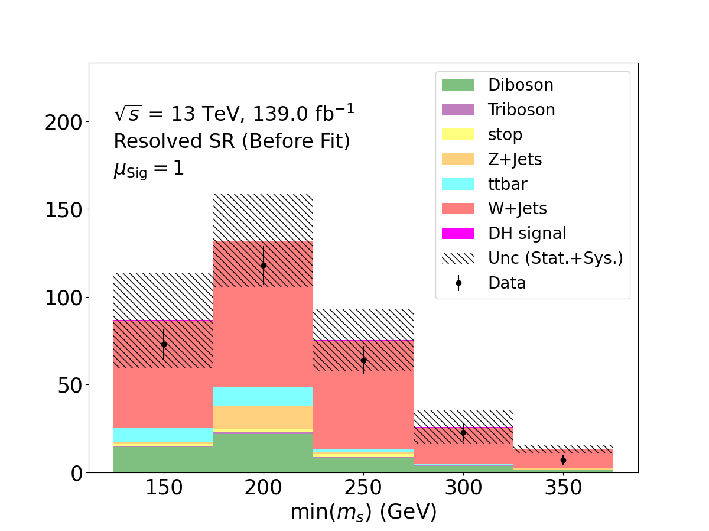
\includegraphics[width=\textwidth]{Figures/8/MonoSlep_monoSWWsemilep_zp2900_dm200_dh310/SR_Resolved_before.pdf}
    \caption{Resolved SR (Before Fit)}\label{fig:before_SR_merged_MonoSlep_monoSWWsemilep_zp2900_dm200_dh310}
  \end{subfigure} \hspace{1em}
  \begin{subfigure}{0.45\textwidth}
    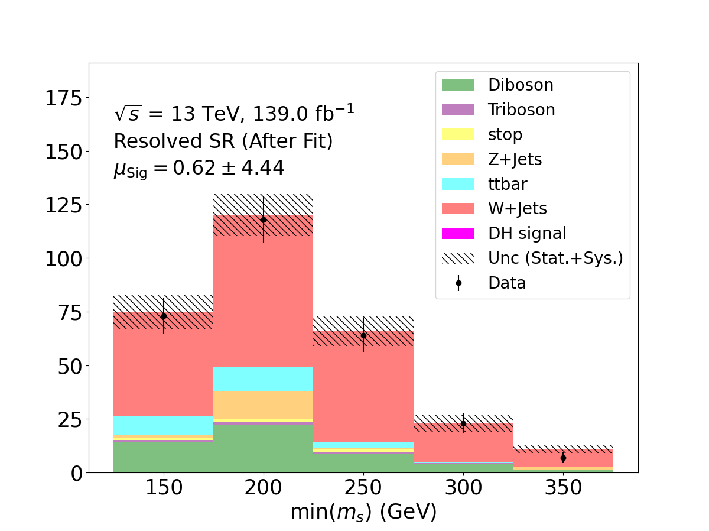
\includegraphics[width=\textwidth]{Figures/8/MonoSlep_monoSWWsemilep_zp2900_dm200_dh310/SR_Resolved_after.pdf}
    \caption{Resolved SR (After Fit)}\label{fig:after_SR_merged_MonoSlep_monoSWWsemilep_zp2900_dm200_dh310}
  \end{subfigure} \\ \vspace{1em}
  \caption[]{Comparison between predicted yields of SM background processes, the DH signal process at \((\ms, \mZp) = (310, 2900)~\GeV\) and observed yields in the SRs. Yields are shown before (left) and after (right) the signal+background fit.}
  \label{fig:before_after_SRs_MonoSlep_monoSWWsemilep_zp2900_dm200_dh310}
\end{figure}


\begin{figure}[H]
  \centering
  \begin{subfigure}{0.49\textwidth}
    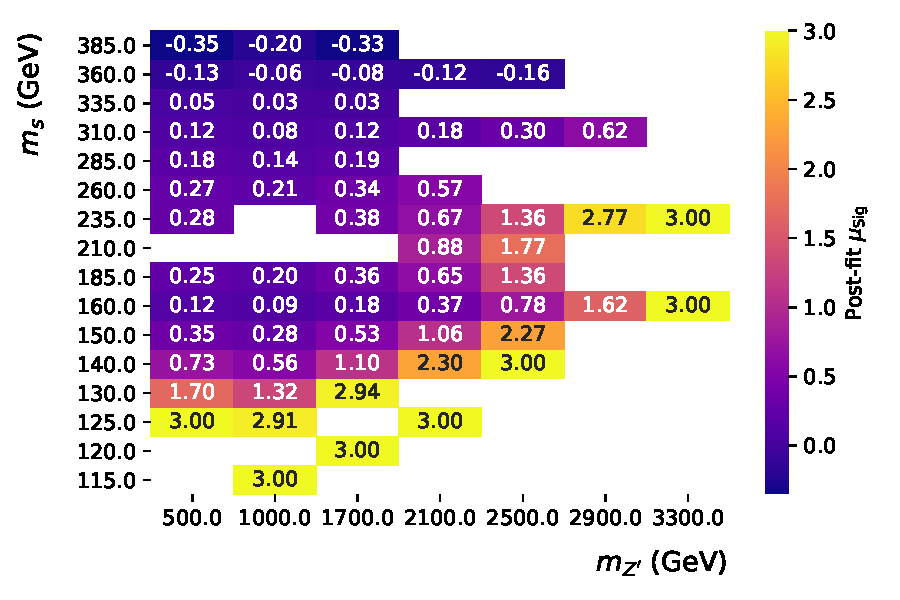
\includegraphics[width=\textwidth]{Figures/8/mu_sigs.pdf}
    \caption{Post-fit \(\mu_\text{Sig}\)}\label{fig:fitted_mu_Sig}
  \end{subfigure} 
  \begin{subfigure}{0.49\textwidth}
    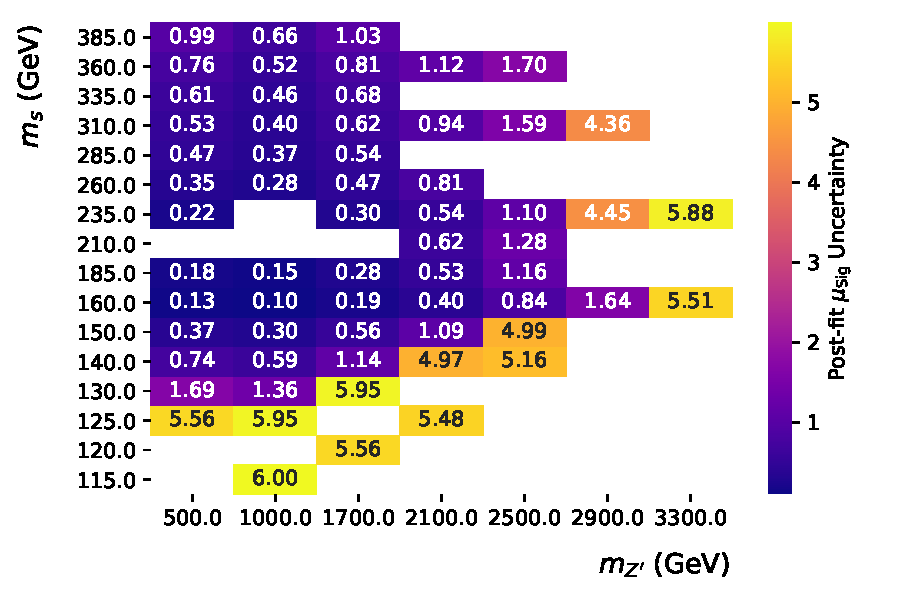
\includegraphics[width=\textwidth]{Figures/8/mu_sig_unc.pdf}
    \caption{Post-fit \(\mu_\text{Sig}\) uncertainty}\label{fig:fitted_mu_Sig_unc}
  \end{subfigure} 
  \caption[]{Post-fit value (left) and uncertainty (right) of the signal strength parameter \(\mu_\text{Sig}\) in the signal+background fit (\(\mu_\text{Sig}\) left floating) for each \ms and \mZp in the DH signal model.}
  \label{fig:fitted_mu_Sig}
\end{figure}

\subsubsection{Nuisance Parameter Pulls and Correlations}

\begin{figure}[H]
  \centering
  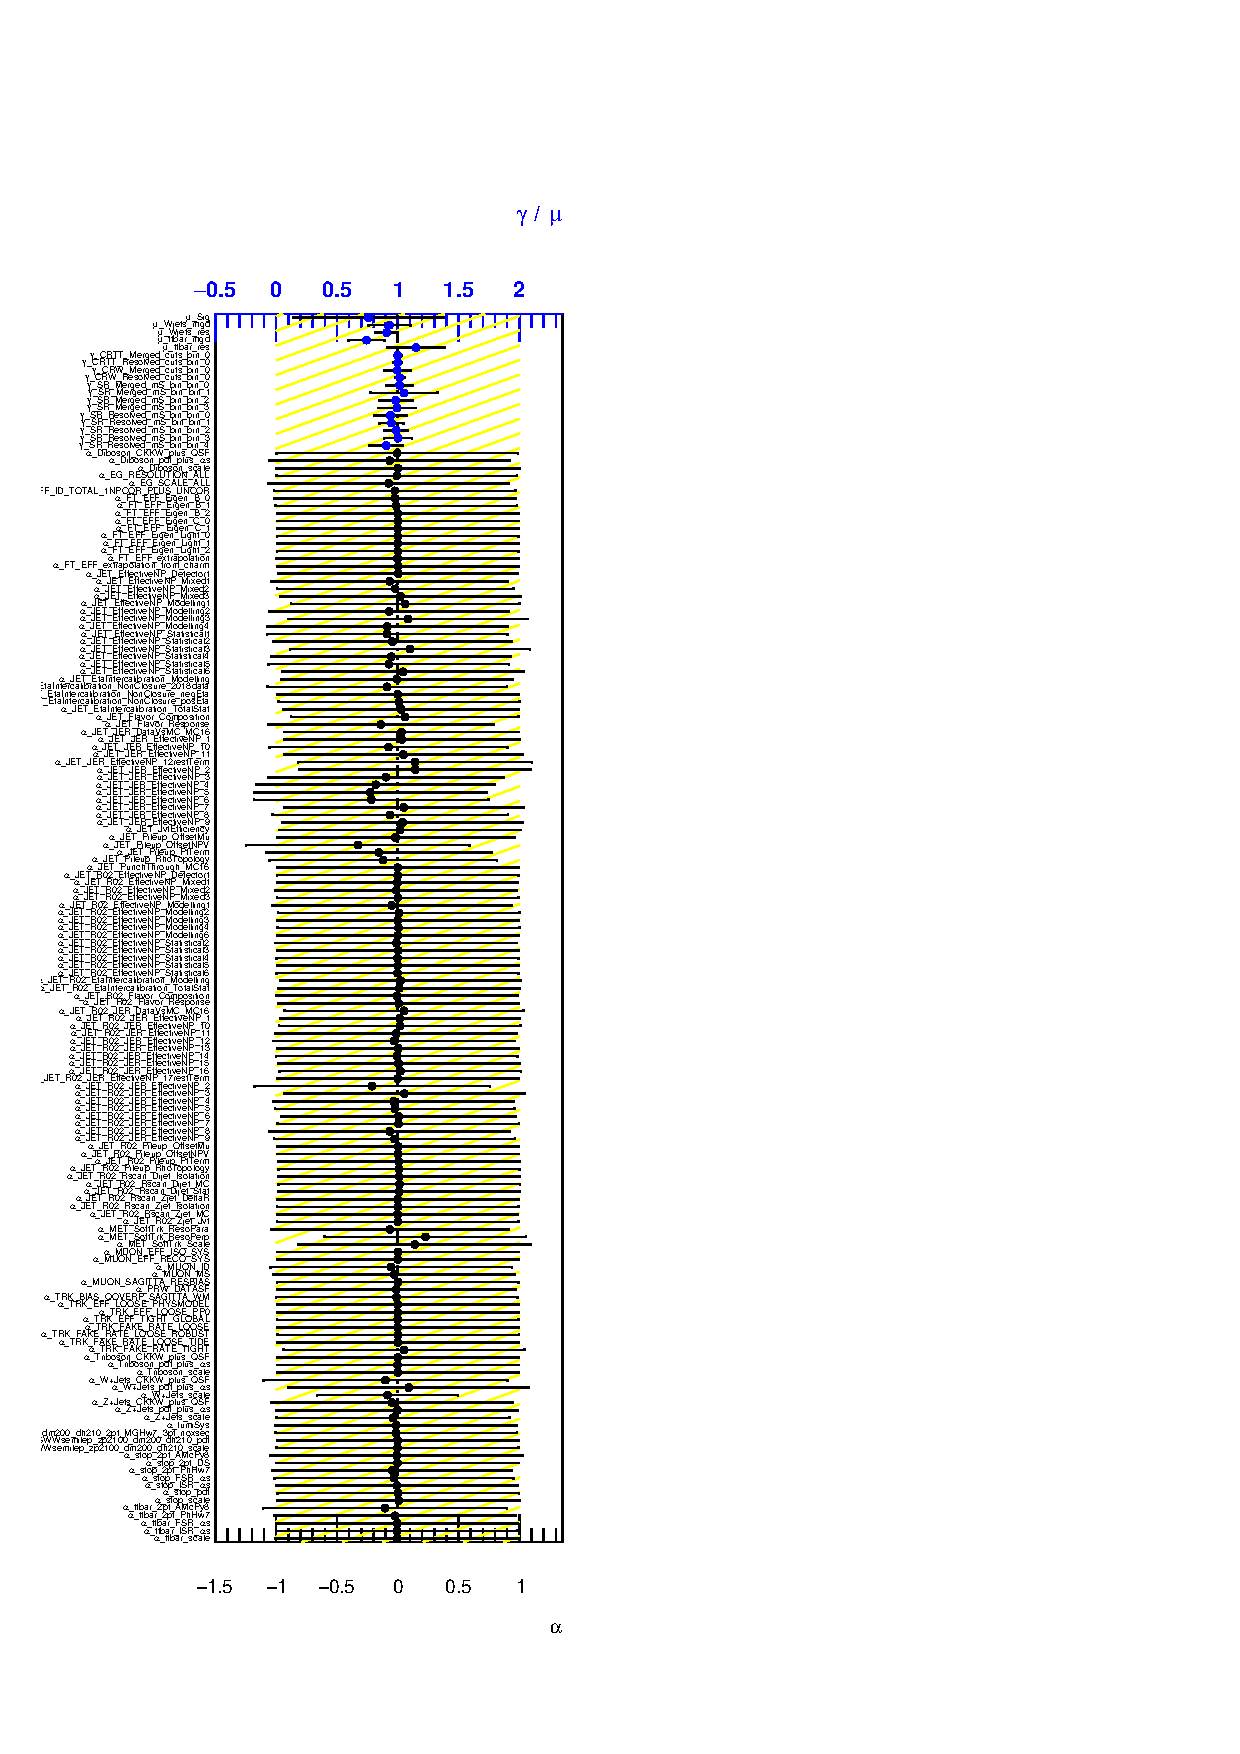
\includegraphics[width=0.5\textwidth]{Figures/8/MonoSlep_monoSWWsemilep_zp2100_dm200_dh210/fit_parameters.pdf}
  \caption[Pull plots for blinded SRs]{\footnotesize{Post-fit values of all NPs in the signal+background fit at a sample signal point of \((\ms, \mZp) = (210, 2100)~\GeV\). See Tables \ref{tab:np_naming}, \ref{tab:exp_syst_naming} and \ref{tab:theo_syst_naming} for details of the scheme used to name the NPs. Yellow hatched band shows the pre-fit uncertainty for each NP, and black horizontal error bars show the post-fit uncertainty.}}
  \label{fig:pull_sigPlusBkg}
\end{figure}

\begin{figure}[H]
  \centering
  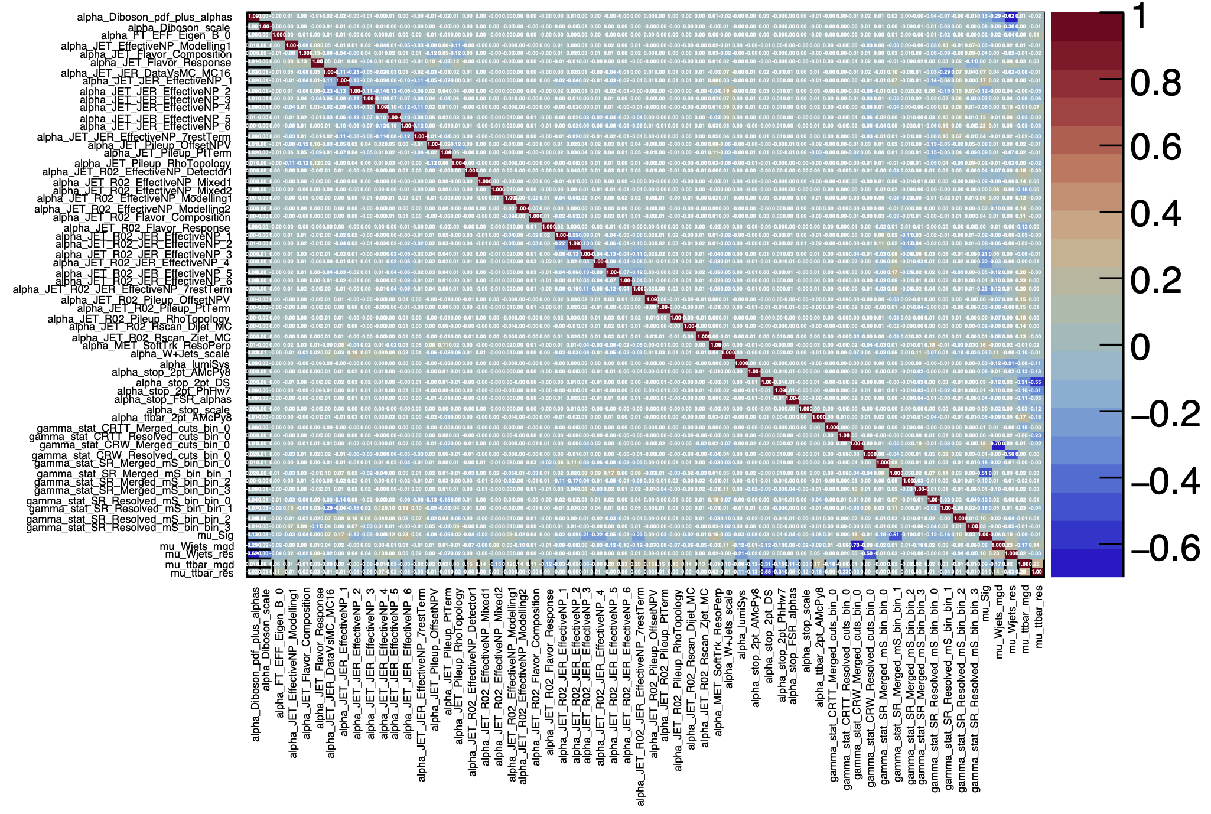
\includegraphics[width=\textwidth]{Figures/8/MonoSlep_monoSWWsemilep_zp2100_dm200_dh210/c_corrMatrix_RooExpandedFitResult_afterFit_edited.pdf}
  \caption[Pull plots for blinded SRs]{\footnotesize{Correlation matrix for all NPs considered in the signal+background fit at a sample signal point of \((\ms, \mZp) = (210, 2100)~\GeV\) for which at least one correlation coefficient with another NP is larger than 0.1. See Tables \ref{tab:np_naming}, \ref{tab:exp_syst_naming} and \ref{tab:theo_syst_naming} for details of the scheme used to name the NPs.}}
  \label{fig:corrs_sigPlusBkg}
\end{figure}

\subsubsection{Ranking of Systematic Uncertainties}

\begin{figure}[H]
  \centering
  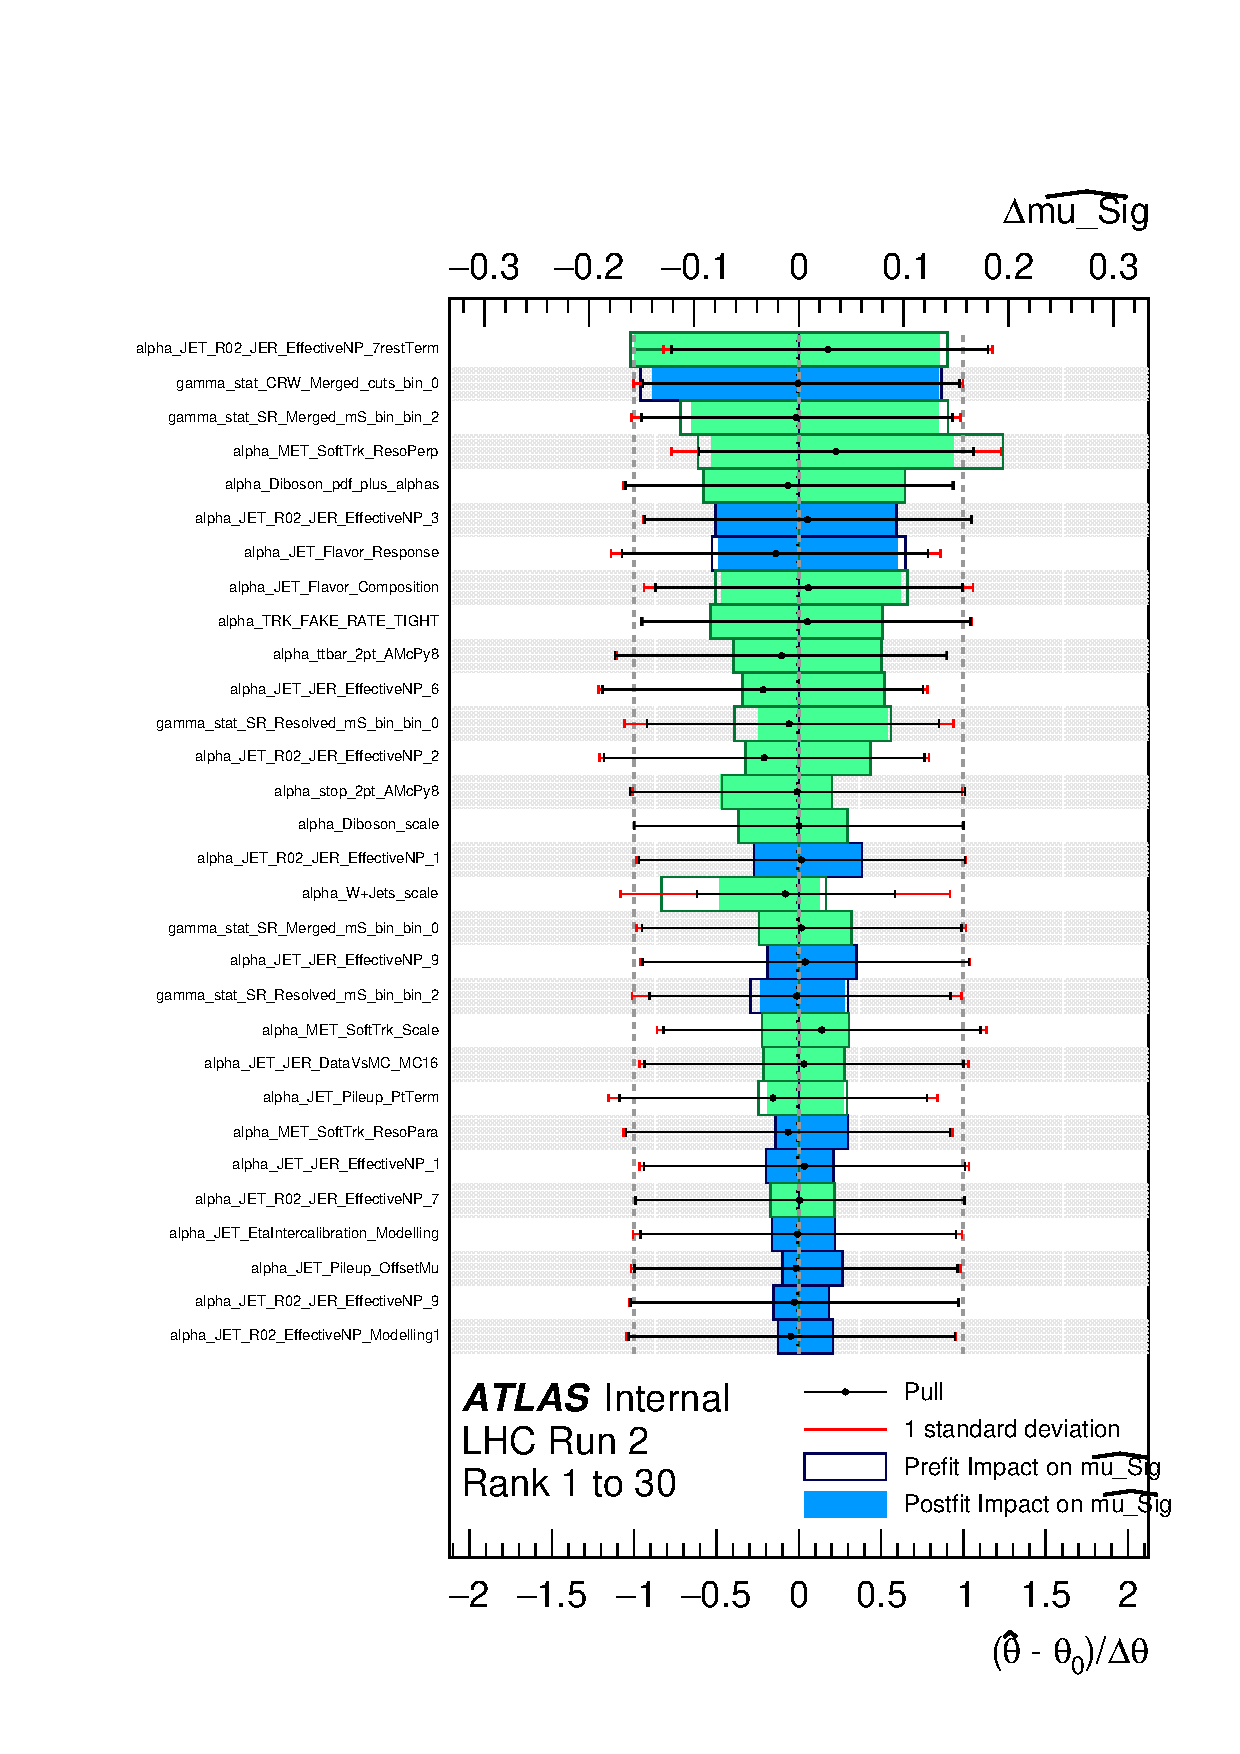
\includegraphics[width=0.9\textwidth]{Figures/8/ranking_mu_Sig_rank_0001_to_0030_zp2100_dm200_dh210_unblinded.pdf}
  \caption[Pre- and post-fit impacts for unblinded CRs (\ms, \mZp)=(210, 2100) GeV]{Leading 30 pre-and post-fit impacts on \(\mu_\text{Sig}\) for nuisance parameters associated with experimental and theoretical uncertainties in the signal+background fit at the sample signal point (\ms, \mZp)=(210, 2100) GeV. NPs are ranked from top to bottom in order of the size of their impact on \(\mu_\text{Sig}\). Blue (green) colouring of post-fit impacts indicates positive (negative) correlation with the signal strength. Red (black) error bars show size of pre-fit (post-fit) uncertainty.}
  \label{fig:ranking_ms210}
\end{figure}

\subsection{Hypothesis Testing and Model Exclusion}

\begin{figure}[H]
  \centering
  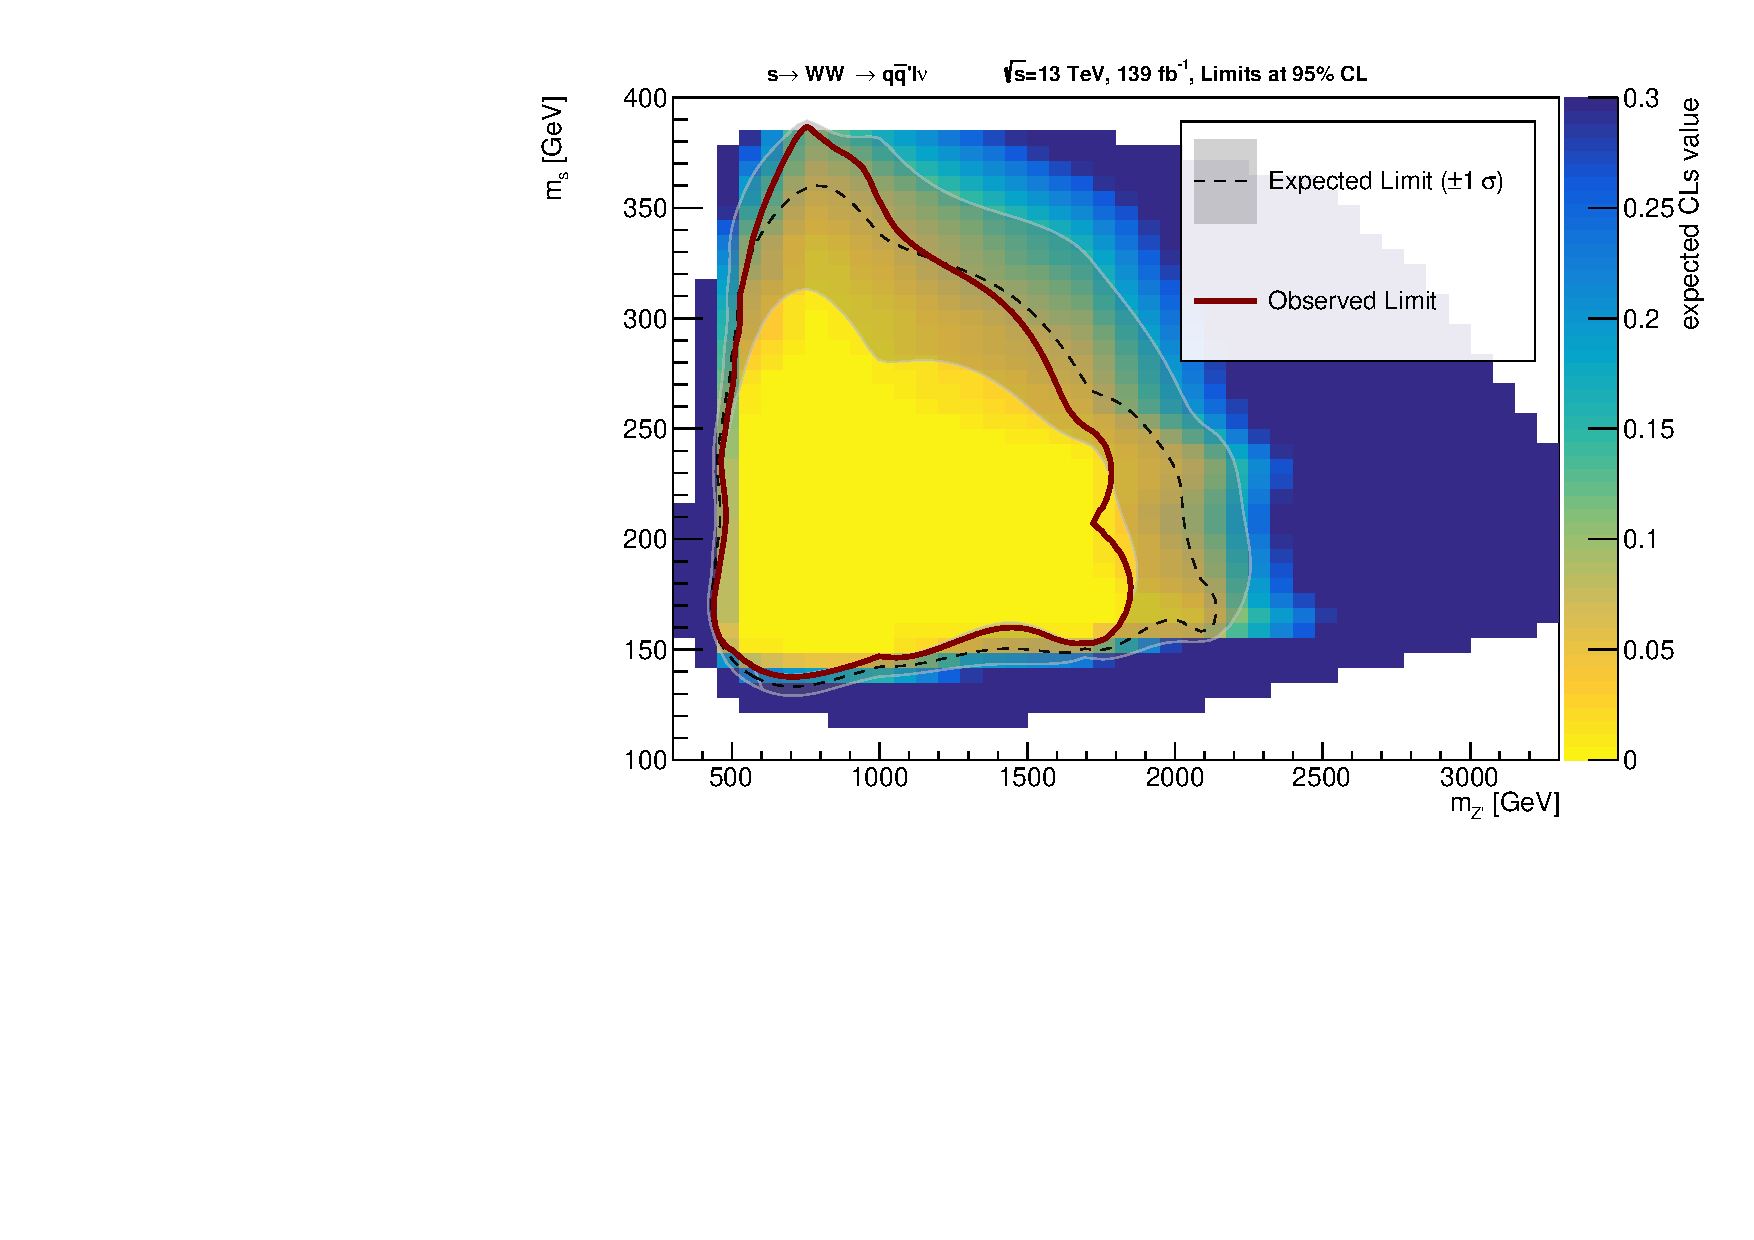
\includegraphics[width=0.8\textwidth]{Figures/8/unblinded_nosig.pdf}
  \caption[]{Projected (grey dashed with \(\pm1\sigma\) uncertainty band) and observed (solid red) range of \ms and \mZp in the DH model excluded by this search. All \ms and \mZp contained within the solid red line are excluded by the search for the choice of \(\sin\theta=0.01\), \(\gchi=1.0\) and \(g_q=0.25\).}
  \label{fig:limits}
\end{figure}

\begin{figure}[H]
  \centering
  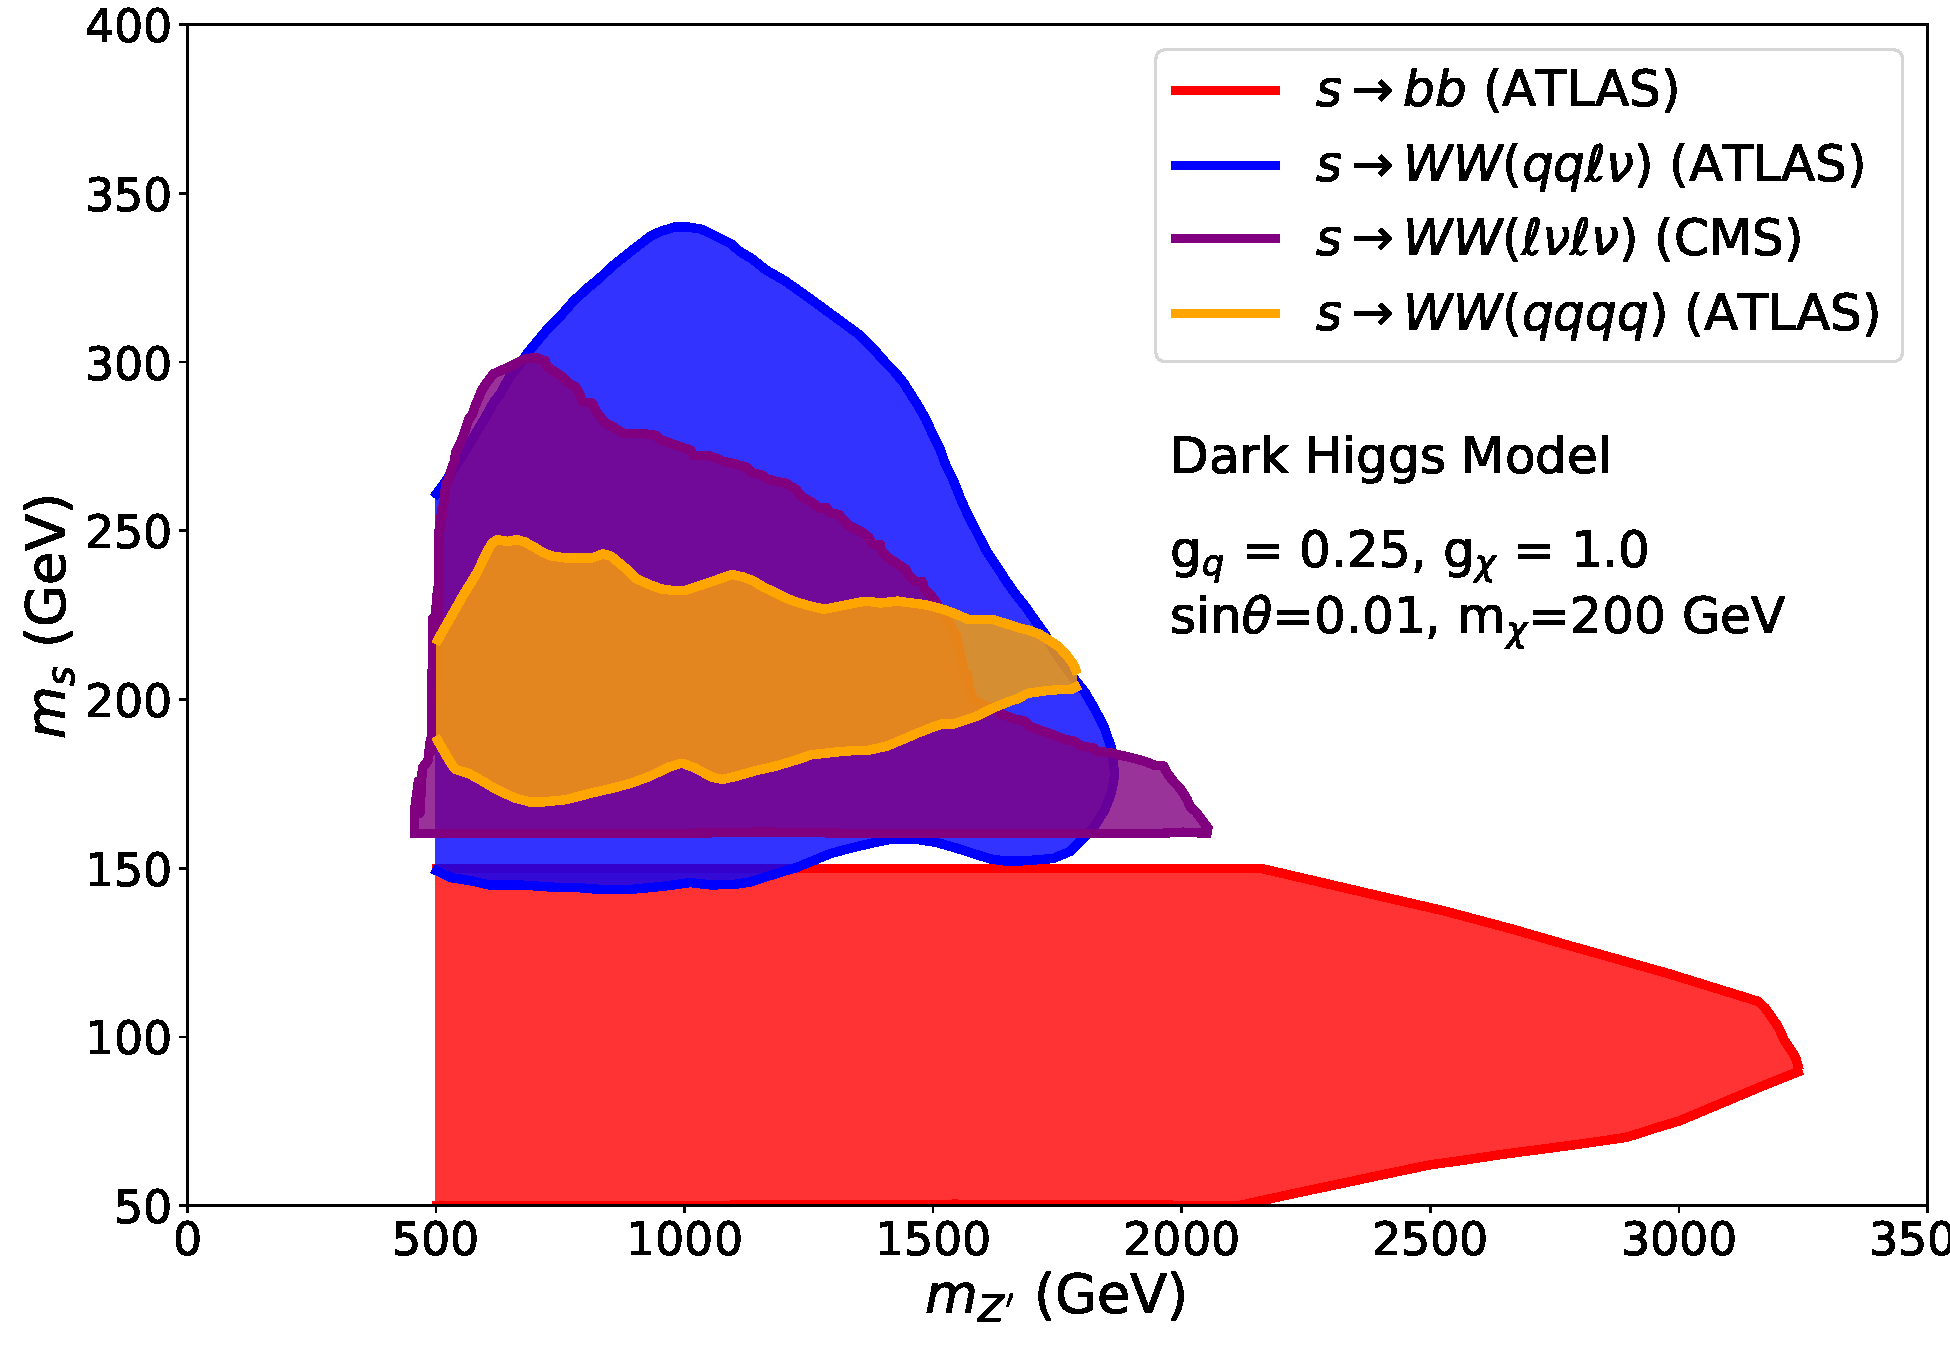
\includegraphics[width=0.8\textwidth]{Figures/8/combined_contour.pdf}
  \caption[]{Summary of \ms and \mZp parameters in the Dark Higgs model excluded by all searches for the model by ATLAS and CMS. All values of \ms and \mZp contained within a coloured area are excluded. The range excluded by the search presented in this thesis is shown in blue.}
  \label{fig:limits_comparison}
\end{figure}


